
\chapter{Motivation}
\begin{verse}
Perhaps chess is the wrong game for the times. Poker is now everywhere, as amateurs dream of winning millions and being on television for playing a card game whose complexities can be detailed on a single piece of paper. But while chess is a 100 percent information game - both players are aware of all the data all the time- and therefore directly susceptible to computing power, poker has hidden cards and variable stakes, creating critical roles for chance, bluffing, and risk management.

These might seem to be aspects of poker based entirely on human psychology and therefore invulnerable to computer incursion. A machine can trivially calculate the odds of every hand, but what to make of an opponent with poor odds making a large bet? 
\end{verse}
\textit{The Chess Master and the Computer} by Garry Kasparov, 2009

\section{Poker and A.I. Research}
Poker is a complex game involving uncertainty, chance and the requirement for strategic and game-theoretic reasoning. Playing this game well, requires the use of intricate strategies as well as a fond knowledge of the stochastic foundations of the game. 

Novice players might see poker as a pure game of chance and look for strategies that play each hand according to its chance of being the best hand in play. This completely misses the fact that the presence of imperfect information allow the usage of advanced strategies, to hide and misrepresent information about a players own card, and trying to win a pot without holding the strongest hand.

The two features of stochasticity and imperfect information have made poker an interesting field for A.I. research. Thanks to a recent boom of poker and computer poker research as well, regular computer poker competitions ( \cite{TheAnualComputerPokerCompetition2010} and  human-computer matches (\cite{TheFirstManMachinePokerChampionship2007},\cite{TheSecondManMachinePokerCompetition2008}) are conduected.

There has been a recent flurry of research into developing strong programs for playing poker. Just as chess was once seen as an important challenge problem for AI, poker is now starting to be seen in the same way. Research has progressed to a point where Heads-Up Limit Hold'em programs have shown performances capable of winning against some of the best professional poker players. 

Thanks to various characteristics, poker is a appropriate testbed to apply concepts of artificial intelligence. The most important ones, according to \cite{Schauenberg2006} thereby are: 

\begin{itemize}
	\item \textit{decision-theory and probabilistic reasoning} - The randomness from the deal of cards and the lack of knowledge of the opponents cards make poker a noisy and uncertain domain. This forces a player to be adept at both decision-theory and probabilistic reasoning.
\item  \textit{risk assessment} - Poker is played in stages containing both the deal of additional cards and wagering. To be able to handle this type of domain of chance, a successful player must be able to assess risks.
\item \textit{opponent modeling} - In poker each hand represents a repeated against the same adaptive agent. This type of environment allows a player to use opponent modeling to
learn their opponents playing strategies and attempt to exploit this knowledge to increase their profit.
\end{itemize}

Most of these aspects can also be found in other fields of artificial intelligence, with the chance of carrying over insights gained by computer poke into other realms, such as: 


\begin{itemize}
\item \textit{user modeling} - Opponent modeling is a form of user modeling. As such, its a recurring problem of modern A.I. research.

In typical user modeling research, a observer tries to find patterns in the behavior of an observed entity. The identified patterns can then be used to customize an application to take advantage of the identified user preferences.

\item \textit{policy-making or negotiation agents} - Game theorists long ago realized poker could be used to illustrate fundamental principles of game theory that have subsequently been applied to a variety of fields including law, politics and economics. 

The development of automated decision-making in poker could lead to advancements in creating tools for use in these domains.
\end{itemize}

The bulk of the research into computer poker, including that from the University of Alberta - currently one of the driving forces in this field, has been on Heads-Up Limit Texas Hold'em. In this game, the players only ever have at most three possible actions (fold, call, or raise). In No-Limit Texas Hold'em on the other hand, players may bet any amount up to the amount of chips remaining in their stack. This rule change significantly alters the optimal strategies, and also poses new research problems when developing a computer program for playing the game. 

For this reason and the fact that No-Limit Poker has become much more popular in the last few years his thesis will focus on the No-Limit variant - though most approaches can also be and have been used in Limit Poker.

\section{Texas Hold'em Poker Rules}
\subsection{Betting structures}

Texas Hold'em is normally played with small and big blinds and the possibility for antes. These forced contributions by the players next to dealer (blinds) or everyone (antes) provide a starting pot to win. 

A dealer button is used to represent the player in the dealer position; the dealer button rotates clockwise after each hand, changing the position of the dealer and blinds. The small blind is posted by the player to the left of the dealer and is usually equal to half of the big blind. The big blind, posted by the player to the left of the small blind, is equal to the minimum bet. In tournament poker, the blind/ante structure periodically increases as the tournament progresses, so players are forced to amass more and more chips to stay in the tournament.

When only playing with two players, e.g. at the end of a tournament, special 'heads-up' rules are enforced and the blinds are posted differently. In this case, the person with the dealer button posts the small blind, while the other player off the button places the big blind. Since the big blind has option, the dealer acts first before the flop. After the flop, the dealer acts last (as normal) and continues to do so for the remainder of the hand.

There�s no one rule of how to set up the betting in all games of poker. The four most common various of Texas Hold'em are limit, spread limit, pot limit and no limit.

\begin{itemize}
\item \textit{Limit} Hold'em has historically been the most popular form of Hold'em found in casino live action games in the United States. In limit Hold'em, bets and raises during the first two rounds of betting (pre-flop and flop) must be equal to the big blind; this amount is called the small bet. In the next two rounds of betting (turn and river), bets and raises must be equal to twice the big blind; this amount is called the big bet. 
\item \textit{Spread limit} is often played in home games. In a spread-limit game, a player can bet any amount within some range � for instance \$1-\$5. This results in a game where the minimum any player can bet is \$1, and the most anyone can bet or raise at one time is \$5. If someone wishes to re-raise, they must raise at least the amount of the previous raise. This minimal raise rule also holds true for pot-limit and no-limit.
\item In \textit{pot-limit} Hold'em, the maximum raise is the current size of the pot (including the amount needed to call). Other then that, all bets and raises are allowed.
\item \textit{No-Limit} Hold'em is the form most commonly found in tournament poker and is currently probably the most popular variant. In No-Limit Hold'em, players may bet or raise any amount over the minimum raise up to all of the chips the player has at the table (called an all-in bet). The initial minimum raise is equal to the big blind. 
\end{itemize}

\subsection{Play of the hand}

At the begin of each hand of Texas Hold'em, all players are dealt two cards face down, starting with the player left of the dealer (the small blind). Texas Hold'em is played with a standard 52-card deck containing no jokers. The two hidden cards are called the players hole cards. They are the only cards each player receives individually and they will only be revealed if a showdown occurs or a player shows them voluntarily after finishing the hand. 

The game begins with a pre-flop betting round, beginning with the player left of the big blind and continuing clockwise. In a betting round, each player is asked to act, either checking (passing on the action, if no call is required),  betting (placing a wager), calling (even another players bet) or raise (call a bet, and further bet an additional amount).

 A round of betting continues until every player has folded, put in all of their chips, or matched the amount put in by all other active players. The blinds are considered "live" in the pre-flop betting round, meaning that they contribute to the amount that the blind player must contribute, and that, if all players call around to the player in the big blind position, that player may either check or raise (or call/fold).

After the pre-flop betting round, assuming there remain at least two players taking part in the hand, the dealer deals a flop, three face-up community cards. The flop is followed by a second betting round. This and all subsequent betting rounds begin with the player to the dealer's left and continue clockwise.

After the flop betting round ends, a single community card (called the turn or fourth street) is dealt, followed by a third betting round. A final single community card (called the river or fifth street) is then dealt, followed by a fourth betting round. If at this point of the game, more than one players remain, each shows his hands (or mucks, if he surrenders the pot) and the pot is awarded to the player with the strongest hand.

\subsection{The showdown}

If a player bets and all other players fold, then the remaining player is awarded the pot and is not required to show his hole cards. If two or more players remain after the final stage, a showdown occurs. On the showdown, each player plays the best poker hand they can make from the seven cards comprising his two hole cards and the five community cards. A player may use both of his own two hole cards, only one, or none at all, to form his final five-card hand. If a player decided to surrender the hand (since another player might already have shown a stronger hand) he can muck his hand without showing, losing any right to the pot.

If the best hand is shared by more than one player, then the pot is split equally among them, with any extra chips going to the first players after the button in clockwise order.

\section{Related Work}
\label{s:relatedwork}

There are various ways to tackle the problems posed by Poker. This section will summarize the most common approaches used in the past and present. The methods involving game tree search will be thoroughly explained in the next chapter. 

\subsection{Expert System}
In a heuristic-based approach to playing poker a rule-based expert system is used to make a poker betting decision. To make a decision, the expert system first abstracts a complicated game state into some simplified scenario that has one or more heuristics (e.g. opponent behavior, a players hole cards and/or the public board texture) associated with it and then it uses that heuristic information to make a decision.

A heuristic based approach is appealing for novices of the game since it's possible to formulate simple rules to base ones play upon. There is a plethora of poker literature focusing on this approach by explaining the heuristics a player should spend attention to, and how to react to common game scenarios given these heuristics. Examples of this approach are hand-ranges to play or fold in the pre-flop stage or strategies to disguise ones hand. As these rule sets are inherently easy to reuse, they offer a natural starting point for building poker-playing programs. 

There are different ways to compile the heuristics which govern these betting strategies. As mentioned, they could be compiled by a domain expert (e.g. a professional poker player or book author), or another way would be to derive and refine computationally through trial and error. Like most rule-based artificial intelligence algorithms, these rule-sets unfortunately quickly become too large to further develop and test. This also holds true for poker, where a situation rarely occurs twice - and the required style of play can differ a lot between different opponents, so it's hard to find rules covering all possibilities that might occur during a game.

Nevertheless, due to the perceived simplicity, this approach was used for various implementations of poker-playing program. As reported, \cite{Waterman1970} attempted to learn production rules to define a betting system for 5-card draw poker. His program reportedly achieved roughly the level of play of an experienced human player. \cite{Smith1983} later revisited the same problem and achieved comparable performance in 5-card draw poker, despite using less domain knowledge. It has to be mentioned though, that 5-card Draw, quite popular at that time, is not as strategically complex as other poker games, like Texas Hold'em (\cite{Sklansky1999}).

\cite{Korb1999} created a computer player for heads-up 5-card stud poker. His player used a Bayes' Network to provide an heuristic betting strategy, enriched with opponent information to provide a better estimate of the winning chance of a hand. This player won against two simplistic test opponents, but lost against an amateur poker player.

The University of Alberta Poker Research Group, a strong driver of computer research, also developed two heuristic-based programs. In these two programs called Loki (\cite{Papp1998} and \cite{Davidson2002}), opponent modeling information was used to increase the accuracy of the computed hand strength and hand potential values on which their their expert-defined formula-based betting strategy based its strategy. These programs have shown an impressive performance in full-ring Texas Hold'em games. In the limit variance of the game they were crafted for, they achieved the level of an intermediate human player. 

Still, \cite{Davidson2002} concluded that these approaches won't scale to world-class play. They too believed that poker has to many different decision scenarios to be be sufficiently handled by any knowledge-engineered heuristic-based betting strategy. Another shortcoming was, that to debug such programs an poker expert was required to identify mistakes in the betting strategy and suggest the improvements necessary.

For this reasons, heuristic-based approaches have mostly been abandoned in academic research. The ease to build them though, makes them still popular for poker-teaching programs and poker bots used to (illegally) profit at low stakes on online poker sites (e.g. \cite{Devlin2008} and \cite{Bornert2009}). 

Poki still remains one of the best ring table players, mostly because research focus has shifted to heads-up poker.

\subsection{Simulation-Based Approaches}
\label{section:simulationbased}

Before the game tree algorithms described in the next chapters were developed, \cite{Billings1999} and \cite{Davidson2002} tried out another way, similar to the game tree search approaches to other game playing problems like chess.  Since game-tree search works so well in these domains, the natural step was to test something analogous to game-tree search in the poker domain.

Game-tree search will be further explained in chapter \ref{c:game-tree-search}. Put short, in most two-player perfect information games it has shown to be effective to search the extensive form of  game-tree several moves ahead, and then call an evaluation function. Unfortunately, in poker the best response for the opponent is unknown because we do not know what cards they are holding. 

Simulation based approaches choose among actions at a certain point of game, and try to simulate the rest of the game to figure out the payout of a certain action. Figure \ref{fig:simulation-vs-search} shows the difference between standard game-tree search algorithms with an evaluation method like alpha-beta (left) and a simulation with selective sampling (right). Unlike alpha-beta, where a full-breadth, but only limited depth search is conducted, simulations search a selection of paths to the leaf nodes of the tree. A technique known as Selective Sampling was used to assign probable values to the unknown variables (the cards of the opponents). Instead of doing a comprehensive but shallow search, a deep but sparse simulation can probe numerous times to the leaves. Each trial of the simulation selectively samples the search space. With enough trials the cumulative selective sample converges to a statistically confident result.

\begin{figure}[!ht]
\centering
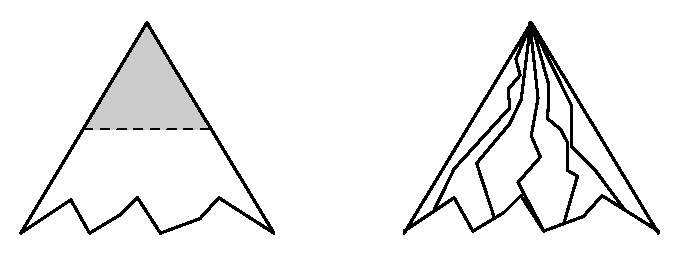
\includegraphics[width=\linewidth]{section02-motivation/figures/simulation-vs-search}
\caption{The difference between classic game-tree search (left) and simulations (right). (\cite{Davidson2002})}
\label{fig:simulation-vs-search}
\end{figure}

In simulation-based Poki by \cite{Davidson2002}, each possible action was simulated by iterating he game to the end of the hand. Since the complete game-state is unknown, probably cards are assigned to each player in each trial of the simulation. After simulating hundreds of trials, an average amount won or lost is known for each action. The action with the largest expected value will then be played by Poki.

The betting strategy according to \cite{Davidson2002} determines the expected values as follows: 

\begin{itemize}
	\item For each trial, probably hands are assigned to each opponent to hold. They also choose hands for players that have already folded, to remove these cards from the deck. For each opponent, a card weight table is maintained throughout the game.
	\item Once each player has a simulated hand assigned, the unknown board cards are randomly chosen from the remaining cards in the deck.
	\item For each trial, the hand is simulated twice. In the first simulation, Poki first calls or checks, in the second Poki would raise of bet (obviously, Poki was used to play limit poker). Once the first action is made, the rest of the hand is simulated to completion. When a simulated opponent must act, their opponent model predicts what he would most likely do in that context. 
	\item Once the simulated hand is finished, the net amount won or lost is recorded.
\end{itemize}

\cite{Davidson2002} reports that in the limited time frame of one or two seconds, around 200-300 trials can be simulated. After this number of trials, the average EV for the different action must have become reasonably stable.

The biggest benefit over rule-based systems outlined before, is that complex strategies can be uncovered without any specific expert knowledge. Tactics such as check-raising, slow playing and bluffing are an emergent property of the simulations. 

Unfortunately, this approach still did not perform as well as hoped. While in ring games, Poki was competitive with intermediate human players, in heads-up games if even lost to very moderate humans. The main reason Poki's simulations did not perform as well as hoped was mostly attributed to the method being extremely dependent on the correct prediction of the opponents future play. Deciding on a single opponent action is extremely difficult, if not impossible, since most opponents also adapt to the situation of the game, and rather think of a distribution of actions to play. By branching at each possible opponent action, the search approach later explained in chapter \ref{c:game-tree-search} takes this into consideration  


\subsection{Game-Theoretic Approaches}
In Game Theory, a nash equilibrium describes a solution of a game, where all players have nothing to gain by changing their own strategy. There can be several different (and possibly infinitely many) equilibria for any given game, but if the game is two-player and zero-sum, every Nash equilibrium provides the same payoffs to all players. In a repeated game where the players change positions, such as heads-up poker, this is a very useful feature - if both players are playing an equilibrium strategy, the expected score for both players will be zero. If one player plays the equilibrium strategy, since their opponent cannot do better by playing a strategy other than the equilibrium, they can expect to at least tie the game.

Unfortunately, due to the complexity of poker (and most other real world games), a equilibrium strategy is rarely achievable. Instead, an approximation of the equilibrium is searched and played - called an  $\epsilon$-Nash equilibrium strategy.  $\epsilon$ is the measure of how far from the actual equilibrium the strategy is. Since a pure equilibrium strategy would loose nor gain more than 0 against any opponent,  $\epsilon$ is the value a best response could win against an  $\epsilon$-equilibrium strategy. Therefore,  $\epsilon$-equilibrium strategies are called suboptimal, or exploitable. But as long as the abstraction is strategically similar to the real game, these strategies can be very difficult to defeat in the full game.

As there are various general-purpose algorithms to calculate equilibria with linear equations, there exist various approaches towards creating $\epsilon$-Nash equilibria agents for poker.

A game theoretic approach results in a approximation of what could be described as "solving" poker, since it searches a generally valid strategy offline, instead of specifically "deciding" what to do in a specific situation during the game. The game theoretic solutions are usually calculated before the game - this limits its ability to adapt to an opponent, but allows for very strong optimization.

\subsubsection{University of Alberta, Edmonton}

The Computer Poker Research Group at the University of Alberta has developed a variety of $\epsilon$-Nash equilibrium strategy agents.

To take the missing information into consideration, the University of Alberta uses a concept they call information sets. A information set contains all possible and indistinguishable states of an opponent in a game tree. All states in the game tree that only differ by the hand an opponent might hold, are therefore collected into one node - a information set. 

Strategies for extensive form games like poker can be represented in several ways. One straightforward way would be to enumerate all possible information sets and record the probabilities of taking each action from that information set.

An alternate method of representing a strategy is to store the probability of playing along each sequence of actions. Considering a sequence of actions by a player and its opponents that have reached a terminal state. Assuming that the player and the opponent play to reach this outcome, we can find the probability of the player selecting their actions in this sequence. This is known as a realization weight.

A set of such realization weights defines a strategy. To find action probabilities at an information set during a game, the sum of the realization weights associated with all reachable terminal nodes after this action can be summed up. 

A linear program can be created to find optimal realization weights subject to constraints (action probabilities are non-negative and sum up to 1). The result is a pair of strategies that are best responses to each other: a Nash equilibrium. 

The \textit{PsOpti} family of programs use an abstract version of the game, which then gets converted into the sequence form. The sequence form then is treated as a series of constraint in a linear program. A solver then can solve these equation system to find an $\epsilon$-Nash equilibrium strategy.

But even after such an abstraction, in the case of the \textit{PsOpti} family of programs, the program needed to solve the entire abstract game was too large to fit into the memory of a computer or a cluster of computers. 

To shrink it, so it could fit into a computers memory, two additional abstractions had to applied. For one thing, they changed the rules of Limit Hold'em so one less bet was allowed on each stage (only two bets or raises Pre-Flop and three on the other stages - \textit{PsOpti} was only playing Limit Hold'em).

Then, seven 3-round Flop strategies were created; each one assumes a different Pre-Flop betting sequence (check-call, check-bet-call, etc) was followed. This combination of strategies could then be used to compose the overall strategy. 

This Pre-Flop strategy was only used on the Pre-Flop. On the flop, a different post-flop strategy was computed and chosen, depending on the observed Pre-Flop action of the player and the opponent.

This disconnect between the Pre-Flop strategy and the strategy used in the rest of the game was a flaw in the \textit{PsOpti} agents that could be exploited by bots with a good opponent model, or by human players aware of this flaw. 

Later Agents tackled that problem by forming one cohesive strategy (\cite{Zinkevich2007b} ) for the whole game or a more robust  $\epsilon$-Nash equilibria approximation (\cite{Johanson2007}). Both approaches saw a immediate increase in performance over the previous \textit{PsOpti1-4} agents.

\textit{Smallbot2298} is another game theoretic approach from University of Alberta. It was produced by a method that does not directly involve solving a linear program, as with the \textit{PsOpti} family of programs and the \textit{GameShrink} approach from the Carnegy Melon University explained later on. Instead, it uses a algorithm described as "Range of Skill" by \cite{Zinkevich2007b}.  It was also one of the first $\epsilon$-Nash equilibrium strategy to use one consistent, whole-game strategy, as opposed to the overlapping strategies used for \textit{PsOpti} and the (first offsprings of the) \textit{GameShrink} family.

The basic idea behind Smallbot2298 is the creation of a sequence of agents, where each one can defeat the agents earlier in the sequence by at least $\epsilon$. For any game and a value for $\epsilon$, this sequence has a maximum length-  sooner or later the sequence approaches within $\epsilon$ of a Nash equilibrium, and no further agents are able to defeat it by more than $\epsilon$. 

To construct this sequence of agents, two algorithms are applied. The first algorithm, \textit{Generalized Best Response I}, considers a game where player 1 is restricted to a set of allowed strategies $S'_1$ while player 2's set $S'_2$ only contains one strategy. A nash equilibrium for this game $G = (S'_{1},S'_{2},u)$ is calculated and the best response for player 2 to player 1 s equilibrium strategy is deducted. This strategy is added to the set $S'_2$ and the algorithm starts again. After enough repetitions, player 2's half of the equilibrium is returned as the best response to player 1's set of strategies $S'_{1}$. 

The second and essential algorithm for this approach, \textit{Range of Skill}, repeatedly calls the generalized best response. After initializing a set of allowed strategies to contain an arbitraty strategy the generalized best response is used to calculate an equilibirum strategy for one player in the restricted game where the other player max only mix between the set of allowed (initially arbitrary) strategies.  This resulting strategy is capable of defeating any of the strategies in the set. 

\begin{lstlisting}[mathescape=true, caption=Algorithm 1: Double Oracle Bundle Algorithm \cite{Zinkevich2007b}]
1. Initialize $S' _1 \subseteq S_1$ and $S'_2 \subseteq S2$. These could be arbitrary singletons.
2. Repeat until satisfied.
2.a) Find a Nash equilibrium $(\sigma_1,\sigma_2)$ in the restricted game $G = (S'_1,S'_2,u)$.
2.b) Compute $BR(\sigma_1)$ and add it to $S'_2$. 
2.c) Compute $BR(\sigma_2)$ and add it to $S'_1$.
3. Return $(\sigma_1, \sigma_2)$.
\end{lstlisting}

\begin{lstlisting}[mathescape=true, caption=Algorithm 2: Generalized Best Response \cite{Zinkevich2007b}]
1. Given $S' _1 \subseteq S_1$, initialize $S' _2 \subseteq S_2$ arbitrarily. 
2. Repeat until satisfied.
2.a) Find a Nash equilibrium  $(\sigma_1,\sigma_2)$ to  $G = (S'_1,S'_2,u)$.
2.b) Compute  $BR(\sigma_1)$ and add it to $S'_2$.
3. Return $\sigma_2$.
\end{lstlisting}

\begin{lstlisting}[mathescape=true, caption=Algorithm 3: Range-Of-Skill Algorithm \cite{Zinkevich2007b}]
1. Initialize $\sum' \subseteq \Delta(S)$ as a singleton. 
2. Repeat until satisfied.
2.a) Find an $\epsilon'$-generalized best response to $\sum' \sigma$.
2.b) Add $\sigma$ to $\sum'$.
3. Return one of the safest mixed strategies $\sum'$ as an $\epsilon$-Nash equilibrium.
\end{lstlisting}

After adding that strategy to the set of allowed strategy, the generalized best response algorithm is called again. Each strategy returned by the generalized best response algorithm in this way is a member of the "range of skill", as each one is capable of defeating the strategies generated before it. The more the sequence of strategies grows, the more the most recent strategies at the end of the sequence approach a Nash equilibrium.

Memory requirements are both the main advantage and disadvantage of the Range of Skill algorithm. By limiting the players of the abstracted game to picking a fixed set of strategies, it avoids solving a huge linear program for the whole game. By circumventing that problem that has hindered other game theoretic approaches, it was possible to deviate on of the first full-game limit Hold'em strategies, without fragmenting like \textit{PsOpti} and \textit{GameShrink}.

On the other hand, for the Range of Skill algorithm, a huge amount of intermediate data has to be stored. Each intermediate strategy most be kept for use in future steps, e.g. to calculate the utility matrix. This data can be stored on a hard disk as opposed to in RAM (for a linear program), but must still be loaded and unloaded often. For scaling to larger abstractions, this might become a problem as \cite{Johanson2007} mentions.

Like other equilibrium approaches, \cite{Zinkevich2007b} ends on the conclusion that even though an equilibrium is a very safe strategy, its rarely the best (exploitive) strategy when playing against a weaker opponent. Game theoretic equilibrium strategies are always defensive strategies, often without the optimal balance between exploitation and safety.


\subsubsection{Carnegie Mellon University, Pittsburgh}

Gilpin and Sandholm from the Carnegie Mellon University produced various nash equilibrium approximations based on their Game Shrink family of algorithms (\cite{Gilpin2006,Gilpin2006b,Hoda2006,Gilpin2007,Gilpin2007b,Gilpin2008}). The resulting players have repeatedly shown to be competitive opponents in the Annual Computer Poker Competitions.

Although Gilpin and Sandholm use a different terminonoly, they share a common foundation with the \textit{PsOpti} agents of the University of Alberta. In their approach, a hand strength metric is called an ordered signal; instead of cards, the agent receives a signal whose value corresponds to the probability of winning the hand. Instead of the term "bucket" to abstract hands, they use the term information filter, which coarsens the ordered signal into a discrete value.

Both \textit{GS1} and \textit{GS2} compute a truncated $\epsilon$-Nash equilibrium strategy to use in the Pre-Flop and Flop rounds. For \textit{GS1}, this truncated strategy considers the betting and cards on the Pre-Flop and Flop rounds; \textit{GS2} considers the betting and cards on the Pre-Flop, Flop and Turn rounds. Both programs use terminal nodes after this point to represent the estimated outcome of the remaining rounds. GS3 and Tartarian later on focused on full-depth equilibrium (\cite{Gilpin2008}). To truncate the remaining stages in \textit{GS1}, they assume that both player call during the Turn and River rounds - resulting in a simple rollout of the later stages of the game. \textit{GS2} uses an estimate of the betting strategy used by \textit{PsOpti}4, conditioned only on the cards and not the earlier betting, as an estimate for the betting actions by both players on the River.

After the turn, the programs construct a linear program in real time and solve it to find a new equilibrium strategy to use later on. As the pre-flop, flop and turn cards are known, the linear program can use a precomputed abstraction that corresponds to the specific set of community cards. For speed, 135,408 of these precomputed abstractions are calculated offline. This provides a much more precise idea of the hand strength at this point in the game than the past filtered signals (buckets) could provide.

Assuming that the opponent is also playing according to the precomputed strategy, the hand strength can be estimated. The linear program to be solved can thus be designed for the current game state: it considers only the betting history that actually occured and the current  community cards.

This linear program is then solved in a separate process while the game further advances. If the player is asked for an action, the agent interrupts the linear program and an intermediate solution can be queried. 

While this allows the agent to produce actions on demand, there is a danger that, as the LP solution is further refined, this intermediate action is no longer part of the solution to the LP. This is called "falling off the tree" since the opponent played an action the strategy wouldn't have selected. The linear program is unable to suggest future actions after that action. In these cases, the agent simply calls for the remainder of the game. 

The main advantage of this approach is that, in theory, the equilibria strategy for the Turn and River rounds will be more accurate than an equilibria strategy in a normal bucket abstraction since the card information on the turn and river are much more precise.

Unfortunately, there are also several significant disadvantages of this approach. For one, solving the linear program in real-time is a difficult task. Normally, a decision has to be made in a matter of seconds (around one minute per hand in live poker, half of that in online poker and 7 seconds per average hand in the annual computer poker competition). In practice, even generating the linear program cannot be done quickly enough to be used in such a short time span.

Another disadvantage is the split between early game and late game. By assuming that both players will only call during the Turn and the River, the Pre-Flop and Flop strategies don't have a accurate estimation of the value of certain lines of player. The concept of implied odds is completely ignored this way.

Implied odds means, that if a strong hand that is likely to win, the amount of money to win isn't only the current pot, but the bets the opponent most call in future rounds. Since the Turn and River rounds have larger bet increments than the Pre-Flop and Flop, assuming that both players will simply call (as \textit{GS1} does) gives too little utility to strong hands, and too much utility to weak hands. 

Another disadvantage is the assumption that the opponent also plays the same equilibrium strategy as the agent. If the opponent does not follow the same Pre-Flop betting strategy as \textit{GS2} (and playing by a different strategy is very likely), then the linear program  used later in the game assumes an inaccurate strength for the opponents hand. And if the opponent doesn't follow the game tree in the turn and river stages, the linear program has lost all value whatsoever.
